\documentclass[a4paper, 11pt, normalem]{report}

\usepackage{../../../LaTeX-Templates/Notes}
\usepackage{subfiles}

\title{Nuclear and Particle Physics \vspace{-20pt}}
\author{Dr Maitre and Dr Bauer}
\date{\vspace{-15pt}Michaelmas Term 2018 - Epiphany Term 2019}
\rhead{\hyperlink{page.1}{Contents}}

\begin{document}

\maketitle
\tableofcontents

\part{}
\chapter{}

Use these because they are made by God himself:
\url{https://dmaitre.phyip3.dur.ac.uk/notes/NPP/}

\emph{Use these notes only with link above, these will just be additional annotations}

\section{Units}

\begin{example}[Do Broglie Wavelength]
    \begin{align}
        \lambda &= \frac{\hbar}{p} \\
        p &= 20 \text{GeV/c} \\
        l &= 0.05 \hbar c\text{GeV}^{-1} \\
        \hbar c &= 0.19733 \,\text{fm}\;\text{GeV} \equiv 1 \\
        \lambda &= 0.0987 \,\text{fm}
    \end{align}
\end{example}

\section{Kinematics}

High energies mean speed close to c, so use special relativity, and get the Lorentz transforms and Tensors.

\begin{example}[4-Momenta]
    In the rest frame of a particle of mass m, 
    \begin{align}
        p &= (m, \vec{0})
    \end{align}
    How is it in a different frame?
    \begin{align}
        p &= (E,\vec{p}) \\
        p\cdot p &\equiv p^2 = \begin{cases} \text{Rest Frame} & m^2 - \vec{0}^2 - m^2 \\ \text{Other Frames} & E^2 \vec{p}\cdot\vec{p} = E^2 - |\vec{p}|^2 \end{cases} \\
        m^2 &= E^2 - |\vec{p}|^2 \\
        E^2 &= m^c + |\vec{p}|^2 \\
        E &= \sqrt{m^2 + |\vec{p}|^2}
    \end{align}
    Note: there will be factors of c in this, but set to 1, in natural units.
\end{example}

\part{}
\chapter{}
\section{Scattering}
\begin{itemize}
    \item de Broglie Wavelength
        \begin{equation}
            \bar{\lambda} = \frac{\hbar}{p}
        \end{equation}
        \begin{itemize}
            \item higher resolution comes from larger momenta
        \end{itemize}
    \item Elastic scattering - Number and particle type are conserved
    \item Inelastic scattering - Number and particle type are not conserved
    \item Total cross section, 
        \begin{equation}
            \sigma_{tot} = \sigma_{el} + \sigma_{inel} = \frac{\dot{N}}{\phi_aN_b}
        \end{equation}
        \begin{itemize}
            \item $\dot{N}$ - rate of collisions
            \item $\phi_a$ - number density in the beam
            \item $N_b$ - number of targets
        \end{itemize}
    \item 
        \begin{equation}
            \dot{N} = \La \cdot \sigma_{tot}, \La = \phi_aN_b
        \end{equation}
        $\La$ is a purely experimental input, $\sigma_{tot}$ purely theoretical.
        \begin{equation}
            \sigma_{tot} = \int_{\Omega} d\Omega \int_{E_{min}}^{E_{max}} dE\;\frac{d\sigma}{d\Omega\,dE}
        \end{equation}
    \item Fermi's Golden Rule:
        \begin{align}
            \sigma &= \frac{2\pi}{V_a}\big|M_{fi}\big|^2 g(E')V \\
            M_{fi} &= \langle \Psi_f | \Ham_{int} | \Psi_i \rangle \\
            \Psi_i &= \frac{1}{\sqrt{V}} e^{i\unl{p}\cdot\unl{x}} \\
            \Psi_f &= \frac{1}{\sqrt{V}} e^{i\unl{p}'\cdot\unl{x}} \\
            \Ham_{int} &= \frac{z\cdot Ze^2}{\unl{x} - \unl{x}'|}\exp{-M|\unl{x}-\unl{x}'|} \\
            M_{fi} &= \langle \Psi_f | \Ham_{int} | \Psi_i \rangle \\
                   &= \int d^3x \Psi^*_f(\unl{x}) \Ham_{int} \Psi_i(\unl{x}) \\
                   &= \frac{z\cdot Ze^2}{V} \int d^3x e^{i\unl{q}\unl{x}} \frac{e^{-M|\unl{x}-\unl{x}_0|}}{|\unl{x}-\unl{x}_0|} \\
                   &= \frac{4\pi e^2 zZ}{V} e^{iqx_0} \frac{1}{|q|^2 + M^2} \to_{M\to 0} \frac{4\pi e^2 zZ}{V} e^{iqx_0}\frac{1}{|q|^2} \\
            d\sigma &= \frac{2\pi}{V_a} |M_{fi}|^2 dg(E') V = \frac{2\pi}{V_a} \bigg|\frac{4\pi e^2 zZ}{V} e^{ix_0\cdot q} \frac{1}{|q|^2}\bigg|^2 V\frac{V}{(2\pi)^3} |p'|^2 d\Omega \\
            \frac{d\sigma}{d\Omega} &= \frac{4e^4z^2Z^2 E'^2}{|q|^4} = \frac{e^4z^2Z^2}{4E^2\sin^4\left(\frac{\theta}{2}\right)}
        \end{align}
\end{itemize}

\section{Mott Scattering}
The Rutherford scattering formula neglects spin.
Spin is a purely relativistic property that distinguishes fermions ($s=\frac{1}{2}$) from bosons ($s=0,1,\dots$).
So the Mott cross-section can be written as
\begin{align}
    \left(\frac{d\sigma}{d\Omega}\right)_{\text{Mott, no recoil}} &= \left(\frac{d\sigma}{d\Omega}\right)_{\text{Rutherford}} \left(1 - \beta^2\sin^2\left(\frac{\theta}{2}\right)\right), \beta = \frac{v}{c} \\
                                                                  &= \left(\frac{d\sigma}{d\Omega}\right)_{\text{Rutherford}} \cos^2\left(\frac\theta 2\right),~ \lim_{v\to c} 
\end{align}
\begin{itemize}
    \item Spin projection on $\unl{p}$ is called helicity:
        \begin{equation}
            h = \frac{\unl{s}\cdot\unl{p}}{|\unl{s}||\unl{p}|}
        \end{equation}
    \item Exception to this when target carries spin as well
    \item Key points:
        \begin{itemize}
            \item For relativistic projectiles, spin has to be taken into account.
            \item Helicity conservation suppresses backwards scattering.
        \end{itemize}
\end{itemize}

\chapter{}
\section{Nuclear Form Factors}
\begin{itemize}
    \item Pointlike charge distribution
        \begin{equation}
            g(x) = Ze\delta^2(x-x_0)
        \end{equation}
    \item Extended charge distribution
        \begin{equation}
            g(x) = Zef(x)
        \end{equation}
    \item
        \begin{align}
            g(x) &= \int g(y) \delta(x-y) dy - Ze \int f(y) \delta(x-y) dy \\
            \phi(x) &= Ze \int f(y) \frac{1}{|x-y|}dy \\
            \Delta\phi(x) &= -g(x) \\
            \Ham_{int} &= ze\cdot\phi(x) \\
            M_{fi} &= \langle \psi_f | \Ham_{int} | \psi_i \rangle \\
                   &= \frac{e}{V} \int d^3x ~ e^{iq\cdot x} \phi(x), q = p-p' \\
                   &= \frac{e}{V} \int e^{iq\cdot x} d^3x ~ Ze\int f(y) \frac{1}{|x-y|} d^3 y \\
                   &= \frac{Ze^2}{V} \int d^3y ~ f(y) \int d^3x ~ \frac{1}{|q|^2} e^{iq\cdot x} \underbrace{\bigtriangleup \frac{1}{|x-y|}}_{...\delta(x-y)} \\
                   &= \frac{Ze^2}{V} \int d^3y~ f(y) \frac{4\pi}{|q|^2} e^{iq\cdot y} \\
                   &= \frac{4\pi Ze^2}{V|q|^2}  \int d^3y ~ f(y)e^{iq\cdot y} \equiv \frac{4\pi Ze^2}{V|q|^2} F(q) \\
            \implies \left(\frac{d\sigma}{d\Omega}\right) &= \left(\frac{d\sigma}{d\Omega}\right)_{\text{Mott, point, no recoil}} |F(q)|^2
        \end{align}
    \item For point-like target, $F(q) = 1$.
    \item The shape of $F(q)$ yields information about the charge distribution. 
        \begin{itemize}
            \item $F(q)$ is the Fourier transform of $f(y)$.
            \item e.g. spherically symmetric target, $f(x) = f(|x|)$
        \end{itemize}
        \begin{align}
            F(q) &= \int e^{iq\cdot x} f(x)\,d^3x = \int f(v) e^{iqv\cos\theta} 2\pi v^2 dv d\cos\theta \\
                 &= \int_v \left(\frac{1}{iqv} e^{iqv\cos\theta}\right)^1_{-1} f(v) 2\pi v^2 dv \\
                 &= \int_v \frac{1}{iqv} \left(e^{iqv} - e^{-iqv}\right) f(v) v^2 dv \\
                 &= 2\pi \int 2 \frac{\sin(qv)}{qv} f(v) v^2 dv \\
                 &= 4\pi \int^1_0 \frac{\sin(qv)}{qv} \left(\frac{3}{4\pi R^3}\right) v^2 dv \\
                 &= \frac{3}{R^3q^3} \left(\sin(qR) - qR\cos(qR)\right)
        \end{align}
    \item Something about graphs leading to $R \approx \frac{4.5}{q_0}$.
\end{itemize}
\begin{figure}[H]
    \centering
    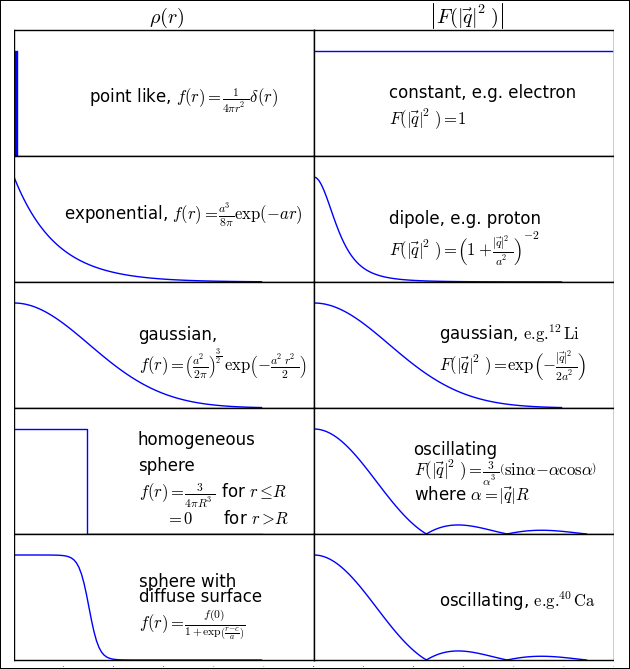
\includegraphics[scale=0.5]{distro.png}
\end{figure}
Key points:
\begin{itemize}
    \item Scattering off an extended charge distribution intoeuces a form factor $F(q)$. $F(q)$ is the Fourier transform of the charge distribution. 
    \item Measure the ration between $d\sigma /d\Omega$ in experiment and Mott allows to determine the shape of $F(q)$.
\end{itemize}

\section{Scattering Off Nucleons}
\begin{itemize}
    \item Require a resolution of $1\,fm = 10^{-15}m$ to perceive nucleons
    \item Requires $q = \frac{\hbar c}{\lambda} = 200\,MeV$
    \item $m_p = 938\,MeV$
    \item For such large momenta, the recoil has to be taken into account: $E \neq E'$
        \begin{equation}
            g(E) = \frac{dn}{dE} = \frac{dn}{dE'}\frac{dE'}{dE} \approx \frac{dn}{dE'}\cdot \frac{E'}{E} = g(E')
        \end{equation}
    \item With this modification, now we have recoil
        \begin{equation}
            \left(\frac{d\sigma}{d\Omega}\right)_{\text{Mott, recoil}} = \left(\frac{d\sigma}{d\Omega}\right)_{\text{Mott, no recoil}} \cdot \frac{E'}{E}
        \end{equation}
    \item The target carries spin, and therefore a magnetic moment. 
        \begin{itemize}
            \item Recall, 
                \begin{equation}
                    \mu = I\cdot A = \frac{q}{2m}L
                \end{equation}
        \end{itemize}
    \item For a spinning charge, 
        \begin{equation}
            \mu = g\frac{e}{M}\cdot S, ~S = \frac{1}{2}
        \end{equation}
\end{itemize}









\end{document}
